\documentclass[a4paper,11pt]{article}

\usepackage[utf8]{inputenc}
\usepackage[top=2cm, left = 2cm , right=2cm , bottom=2cm]{geometry}
\usepackage{amsmath}
\usepackage{graphicx}
\usepackage{float}
\usepackage{listings}
\usepackage[brazil]{babel}
\usepackage{multicol}

\usepackage{color}

\definecolor{mygreen}{rgb}{0,0.6,0}
\definecolor{mygray}{rgb}{0.5,0.5,0.5}
\definecolor{mymauve}{rgb}{0.58,0,0.82}

\lstset{
  backgroundcolor=\color{white},   % choose the background color; you must add
                                   % \usepackage{color} or \usepackage{xcolor};
                                   % should come as last argument
  basicstyle=\footnotesize\sffamily,  % the size of the fonts
  breakatwhitespace=false,         % sets if automatic breaks should only happen
                                   % at whitespace
  breaklines=true,                 % sets automatic line breaking
  captionpos=b,                    % sets the caption-position to bottom
  commentstyle=\color{mygreen},    % comment style
  escapeinside={\%*}{*)},          % if you want to add LaTeX within your code
  extendedchars=true,              % lets you use non-ASCII characters; for
                                   % 8-bits encodings only, does not work with
                                   % UTF-8
  frame=single,	                 % adds a frame around the code
  keepspaces=true,                 % keeps spaces in text, useful for keeping
                                   % indentation of code (possibly needs
                                   % columns=flexible)
  keywordstyle=\color{blue},       % keyword style
  language=Matlab,                 % the language of the code
  numbers=left,                    % where to put the line-numbers; possible
                                   % values are (none, left, right)
  numbersep=5pt,                   % how far the line-numbers are from the code
  numberstyle=\tiny\color{mygray}, % the style that is used for the line-numbers
  rulecolor=\color{black},         % if not set, the frame-color may be changed
                                   % on line-breaks within not-black text
                                   % (e.g. comments (green here))
  showspaces=false,                % show spaces everywhere adding particular
                                   % underscores; it overrides
                                   % 'showstringspaces'
  showstringspaces=false,          % underline spaces within strings only
  showtabs=false,                  % show tabs within strings adding particular
                                   % underscores
  stepnumber=2,                    % the step between two line-numbers. If it's
                                   % 1, each line will be numbered
  stringstyle=\color{mymauve},     % string literal style
  tabsize=2,                       % sets default tabsize to 2 spaces
  title=\lstname                   % show the filename of files included with
                                   % \lstinputlisting; also try caption instead
                                   % of title
}

\pagestyle{plain}

\graphicspath{{./Imagens/}}

\begin{document}	

\begin{center}
\textbf{Pré-relatório Experiência 6} \\
\hspace{5pt}
Prof. Marconi Kolm Madrid \\
EA722 - 2017/2
\end{center}

\begin{center}
Danilo Pereira Titato - RA 122541 \\
Giovani Granzotto Oliani - RA 146253 \\
Pedro Gabriel Calixto Mendonça - RA 118363
\end{center}

\textbf{Projeto de realimentação do carro 1}

\begin{lstlisting}
%% Parametros iniciais
s = tf('s');

% Massa dos carros
mc1 = 0.783; % kg
mc2 = 0.582; % kg

% Massa total dos carros
m1 = mc1 + 4 * 0.500; % kg
m2 = mc2 + 4 * 0.500; % kg

% Coeficiente de atrito dos carros
c1 = 3.90; % N/(m/s)
c2 = 2.36; % N/(m/s)

% Constante de mola
k = 338.6; % N/m

% Ganho de hardware
khw = 14732;

N1 = [m2 c2 k];
N2 = [k];
D = [(m1*m2) (c1*m2 + c2*m1) ((m1+m2)*k + c1*c2) ((c1+c2)*k) 0];
\end{lstlisting}

~~~~\textbf{1.}

\begin{lstlisting}
%% Realimentacao - 1
% Implemente as funcoes de transferencia da planta utilizando os valores
% numericos para definir X1(s)/R*(s)

G1 = feedback(khw * N1/D, kv * s);
\end{lstlisting}

~~~~\textbf{2.}

\begin{lstlisting}
%% Realimentacao - 2
% Determine atraves do lugar das raizes (root locus) o valor de kv que
% forneca o maximo amortecimento

rlocus(s * khw * tf(N1, D));
grid on;
\end{lstlisting}

\begin{figure}[H]
\centering
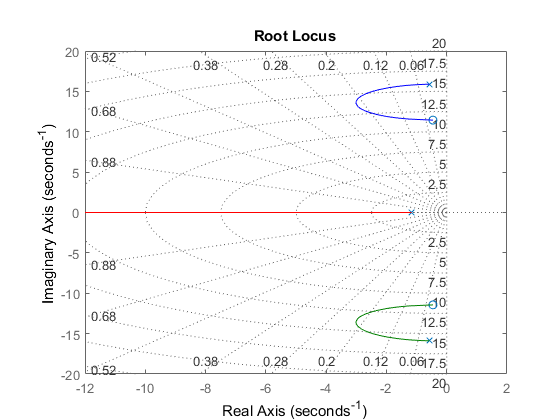
\includegraphics{real-02}
\caption{Lugas das raízes de $X_1\left(s\right)/R^\ast\left(s\right)$}
\end{figure}

Ganho do valor de máximo amortecimento: $gain = 0.00359$. \\

~~~~\textbf{3.}

\begin{lstlisting}
%% Realimentacao - 3
% Implemente kv e determine os polos da funcao de transferencia interna
% G*(s). Selecione os polos complexos conjugados desta f.t., denominando-os
% p1 e p2.

kv = 0.00359;

Gstar = tf(N2, N1) * feedback(khw * tf(N1, D), kv * s);
Gstar = minreal(Gstar);

% obtem o denominador de G*(s), acha suas raizes e filtra aquelas cuja
% parte imaginaria eh diferente de 0 (polos complexos conjugados)
[~, den] = tfdata(Gstar);
p = roots(den{1});
p_id = find(imag(p) ~= 0);
p1 = p(p_id(1));
p2 = p(p_id(2));
\end{lstlisting}

Resultado:

\begin{lstlisting}
p1 = -2.9436 +13.1126i;
p2 = -2.9436 -13.1126i;
\end{lstlisting}

\pagebreak

\textbf{Projeto do filtro notch}

~~~~\textbf{1.}

\begin{lstlisting}
%% Notch - 1
% Calculam-se os parametros do filtro Nn(s)/Dn(s) de modo que:
% 1. os dois zeros do filtro cancelem dois polos de G*(s) (tipicamente
% polos pouco amortecidos), isto eh, raizes de D*(s) complexas conjugadas.

Nn = poly([p1 p2]);

% 2. o filtro possua dois pares de polos complexos conjugados de frequencia
% natural fn1 = 5Hz e fn2 = 8Hz respectivamente, e csi = sqrt(2) / 2 para
% ambos os pares.

csi = sqrt(2) / 2;

wn1 = 5 * 2 * pi; % 5 Hz
wn2 = 8 * 2 * pi; % 8 Hz

% 3. o coeficiente  do  termo  de  maior  grau  do  polinomio Dn(s) deve
% ser 1 (polinomio monico) e o ganho estatico (DC) da funcao de
% transferencia do filtro deve ser unitario.

Dn = conv([1 (2*csi*wn1) wn1^2], [1 (2*csi*wn2) wn2^2]);

Gnotch = tf(Nn, Dn);
Gnotch = Gnotch * (1 / dcgain(Gnotch));
\end{lstlisting}

~~~~\textbf{2.}

\begin{lstlisting}
%% Notch - 2
% Associe G*(s) ao filtro projetado.
G2 = minreal(Gnotch * Gstar);
\end{lstlisting}

\pagebreak

\textbf{Projeto do controlador P\&D}

~~~~\textbf{1.}

\begin{lstlisting}
%% P&D - 1
% Determine atraves do lugar das raizes o valor do ganho kd de forma a se
% obter o maximo amortecimento para os polos dominantes da funcao de
% transferencia da saida x2(t)

rlocus(s * G2);
grid on;
\end{lstlisting}

\begin{figure}[H]
\centering
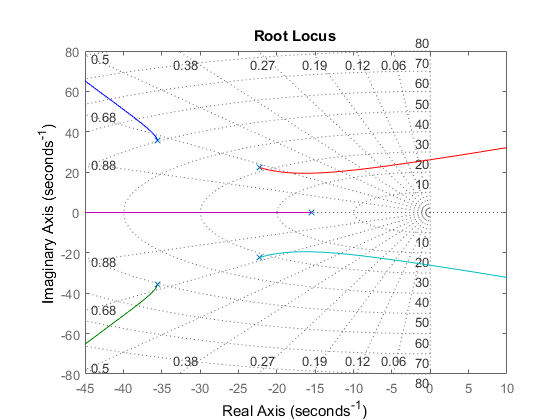
\includegraphics{ped-01}
\end{figure}

Ganho do valor de máximo amortecimento: $gain = 0.00074$. \\

~~~~\textbf{2.}

\begin{lstlisting}
%% P&D - 2
% Implemente o valor de kd e determine atraves do lugar das raizes o valor
% do ganho kp que tenha o minimo tempo de estabelecimento.

kd = 0.00074;

G3 = feedback(G2, kd * s);
rlocus(G3);
grid on;
\end{lstlisting}

\begin{figure}[H]
\centering
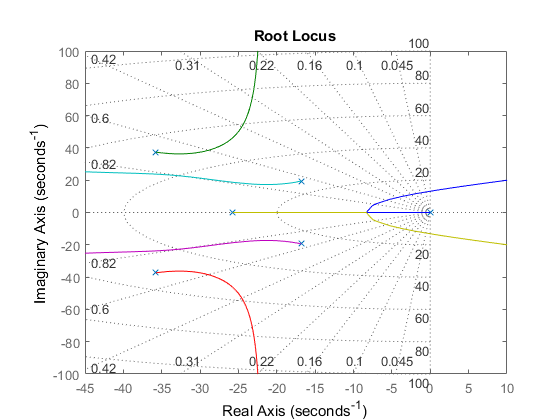
\includegraphics{ped-02}
\end{figure}

Ganho do valor com mínimo tempo de estabelecimento: $gain = 0.0147$. \\

~~~~\textbf{3.}

\begin{lstlisting}
%% P&D - 3
% Utilize a resposta ao degrau do sistema em malha fechada com x2(t) como
% saida, como criterio para verificacao da adequacao do ajuste.

kp = 0.0147;

G = feedback(kp * G3, 1);
step(G);
grid on;
\end{lstlisting}

\begin{figure}[H]
\centering
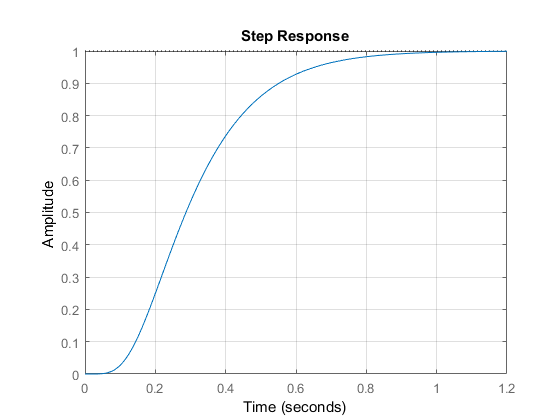
\includegraphics{ped-03}
\caption{Resposta ao degrau do sistema de malha fechada}
\end{figure}

\textbf{Implementação no software ECP}

\begin{figure}[H]
\centering
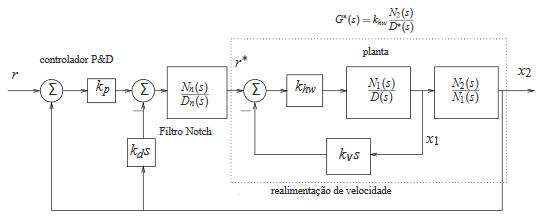
\includegraphics{blocos-01}
\caption{Diagrama para o controle não-co-alocado}
\label{fig:blocos-01}
\end{figure}

Para o diagrama de blocos acima, temos que sua função de transferência se dá
por:

\begin{gather*}
  X_2\left(s\right) = G^\ast\left(s\right) \cdot G_{notch}\left(s\right) \cdot
    \left[k_p \cdot \left(R\left(s\right) - X_2\left(s\right)\right) -
    k_d s \cdot X_2\left(s\right)\right] \\
  X_2\left(s\right) \cdot \left[1 +  G^\ast\left(s\right) \cdot
    G_{notch}\left(s\right) \cdot \left(k_p + k_d s\right)\right] =
    G^\ast\left(s\right) \cdot G_{notch} \cdot k_p \cdot R\left(s\right) \\ \\
  \frac{X_2\left(s\right)}{R\left(s\right)} = \frac{k_p \cdot
    G^\ast\left(s\right) \cdot G_{notch}\left(s\right)}{1 + G^\ast\left(s\right)
    \cdot G_{notch}\left(s\right) \cdot \left(k_p + k_d s\right)}
\end{gather*}

\begin{figure}[H]
\centering
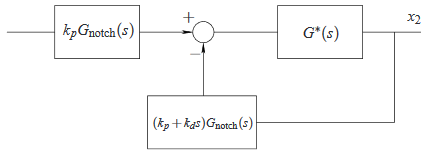
\includegraphics{blocos-02}
\caption{Representação do filtro \textit{notch} + P\&D implementado na malha do
\textit{loop 1}}
\label{fig:blocos-02}
\end{figure}

Para o diagrama de blocos acima, temos que sua função de transferência se dá
por:

\begin{gather*}
  X_2 = \frac{G^\ast\left(s\right)}{1 + G^\ast\left(s\right) \left(k_p +
    k_d s\right) \cdot G_{notch}\left(s\right)} \cdot k_p \cdot
    G_{notch}\left(s\right) \cdot R\left(s\right) \\
  \frac{X_2\left(s\right)}{R\left(s\right)} = \frac{k_p \cdot
    G^\ast\left(s\right) \cdot G_{notch}\left(s\right)}{1 + G^\ast\left(s\right)
    \cdot G_{notch}\left(s\right) \cdot \left(k_p + k_d s\right)}
\end{gather*}

Pode-se ver, então, que a função de transferência do diagrama de blocos da
figura \ref{fig:blocos-01} é igual à função de transferência do diagrama de
blocos da figura \ref{fig:blocos-02}, como queria-se demonstrar.

O bloco correspondente a $k_p G_{notch}\left(s\right)$ se dá na forma
$\frac{t\left(s\right)}{r\left(s\right)}$, enquanto o bloco
$\left(k_p + k_d s\right) G_{notch}\left(s\right)$ se dá como
$\frac{s\left(s\right)}{r\left(s\right)}$. Denotando o numero e o denominador do
filtro \textit{notch} por $n_2 s^2 + n_1 s + n_0$ e
$s^4 + d_3 s^3 + d_2 s^2 + d_1 s + d_0$, temos as seguintes relações entre os
coeficientes dos polinômios:

\begin{multicols}{3}
$t_0 = n_0 k_p$

$t_1 = n_1 k_p$

$t_2 = n_2 k_p$

\columnbreak

$s_0 = n_0 k_p$

$s_1 = n_0 k_d + n_1 k_p$

$s_2 = n_1 k_d + n_2 k_p$

$s_3 = n_2 k_d$

\columnbreak

$r_0 = d_0$

$r_1 = d_1$

$r_2 = d_2$

$r_3 = d_3$

$r_4 = 1$
\end{multicols}

Para o cálculo desses coeficientes $t_i$, $s_i$ e $r_i$, o código Matlab
adicionado foi:

\begin{lstlisting}
%% Calculo dos coeficientes

% Coeficientes do filtro notch
[num, den] = tfdata(Gnotch);

Nn = num{1};
Dn = den{1};

n0 = Nn(5);
n1 = Nn(4);
n2 = Nn(3);

d0 = Dn(5);
d1 = Dn(4);
d2 = Dn(3);
d3 = Dn(2);
d4 = Dn(1);

% Coeficientes dos blocos
t0 = n0*kp;
t1 = n1*kp;
t2 = n2*kp;

s0 = n0*kp;
s1 = n0*kd + n1*kp;
s2 = n1*kd + n2*kp;
s3 = n2*kd;

r0 = d0;
r1 = d1; 
r2 = d2;
r3 = d3;
r4 = 1;
\end{lstlisting}

















\end{document}